\documentclass[a4paper,12pt]{article}
\usepackage[utf8]{inputenc}
\usepackage{amsmath}
\usepackage{amsfonts}
\usepackage{amssymb}
\usepackage{graphicx}
\usepackage{hyperref}
\usepackage{geometry}
\usepackage{fancyhdr}

\pagestyle{fancy}
\fancyhf{}
\renewcommand{\headrulewidth}{0.4pt} % full-width rule
\fancyhead[L]{EEE F313: ADVD Lab 2 Report}
\fancyhead[R]{Pranav Chandra N. V.}
\fancyfoot[C]{\thepage}

\geometry{a4paper, margin=1in}
\title{EEE F313: ADVD Lab 2 Report}
\author{Pranav Chandra N. V. \\ 2023AAPS0013}
\date{}

\begin{document}
\maketitle
\section{Introduction}
This lab had the goal of identifying the noise margins of an NMOS circuit. The VTC curve was plotted of the circuit, and the noise margins were calculated from the graph.
\begin{figure}[h!]
	\centering
	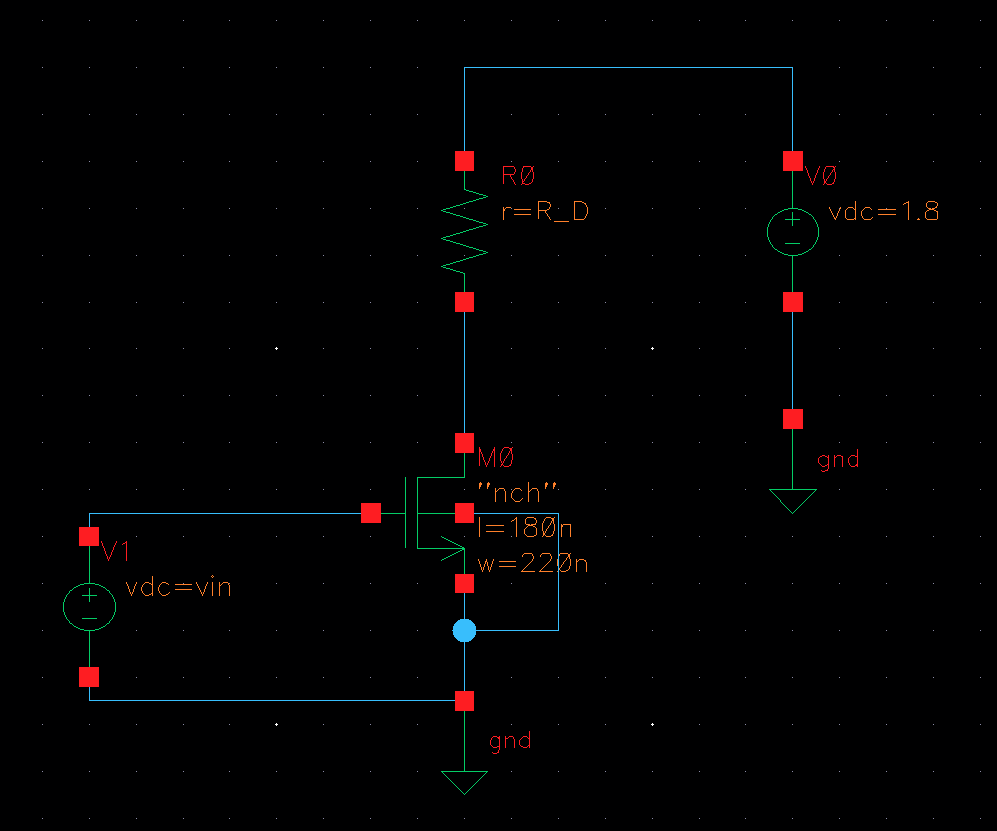
\includegraphics[width=0.8\textwidth]{images/circuit.png}
	\caption{VTC Circuit}
	\label{fig:vtc_circuit}
\end{figure}

Figure \ref{fig:vtc_circuit} shows the circuit used to plot the VTC curve. The values for $V_{in}$ were varied between 0V and 1.8V, with a step size of 0.01V. A DC analysis was plotted, with the NMOS parameters being $l = 180nm$, $w = 220nm$, and $V_{GS} = 1.8V$.

\newpage
\section{Measurements}
The following section describes the measurements achieved from the graph shown in Figure \ref{fig:vtc_curve}. The various lines are explained ni the subsequent subsections.
\begin{figure}[h!]
	\centering
	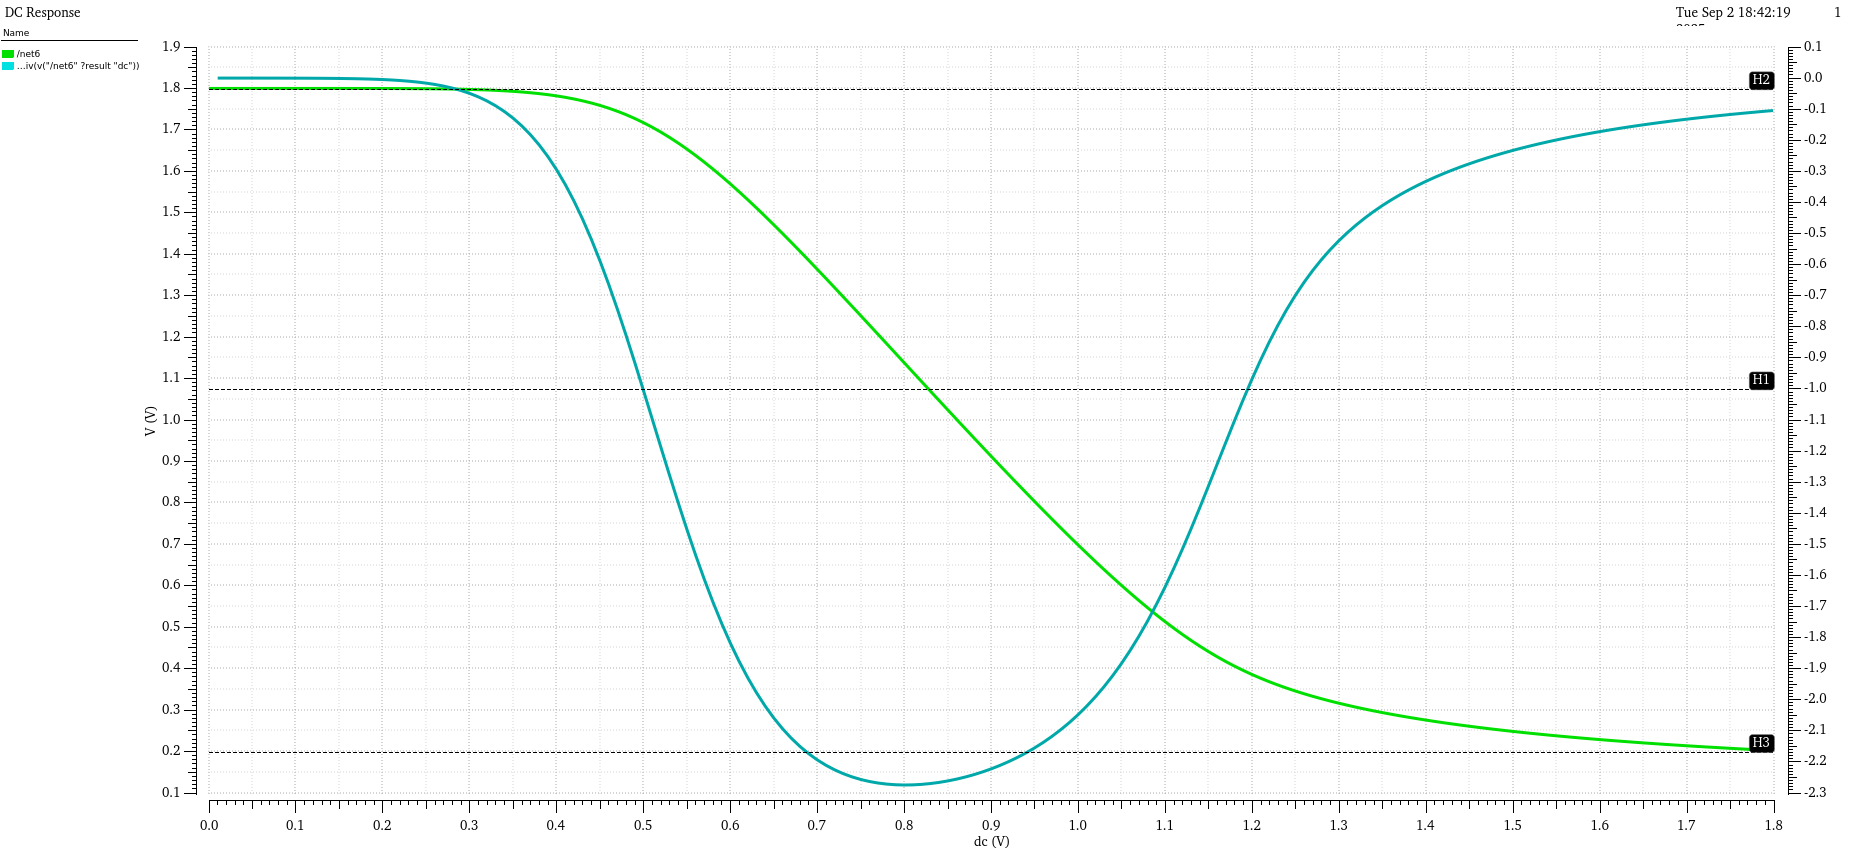
\includegraphics[width=0.8\textwidth]{images/vtc-curve.png}
	\caption{VTC Curve}
	\label{fig:vtc_curve}
\end{figure}

\subsection{Output Voltages}
From the VTC cuve, the following output voltages were measured:
\begin{itemize}
	\item $V_{OH}$ = 1.8V = $V_{DD}$
	\item $V_{OL}$ = 0.2030279 mV $\neq$ GND
\end{itemize}

It's important to note that $V_{OL}$ is not equal to GND, which is a deviation from the ideal case. This is because the NMOS transistor does not pull the output all the way down to GND when it is ON, due to its non-zero resistance.

\subsection{Input Voltages}
The following input voltages were measured from the VTC curve:
\begin{itemize}
	\item $V_{IL}$ = 0.49974 V
	\item $V_{IH}$ = 1.19555 V
\end{itemize}
The voltages were determined by finding the point on the VTC curve where the slope is -1. This was done by taking the derivative of the VTC curve in the cadence software and ientifyng the intersections with the line y = -1.

\newpage
\section{Noise Margins}
The noise margins were calculated using the following formulas:
\begin{align*}
	NM_{L} &= V_{IL} - V_{OL} \\
	NM_{H} &= V_{OH} - V_{IH}
\end{align*}
Substituting the measured values, we get:
\begin{align*}
	NM_{H} &= V_{OH} - V_{IH} = 1.8 - 0.49974 = 0.60445 \\
	NM_{L} &= V_{IL} - V_{OL} = 1.19555 - 0.2030279 = 0.9925221
\end{align*}

\section{Parametric Analysis}
A parametric analysis was done to see the effect of varying the drain resistance (and thus the drain current) on the overall VTC (and thus noise margins) of the circuit. The resistnance was varied from 1k$\Omega$ to 71k$\Omega$ in steps of 10k$\Omega$. The following graph shows the VTC curves for the various resistance values.
\begin{figure}[h!]
	\centering
	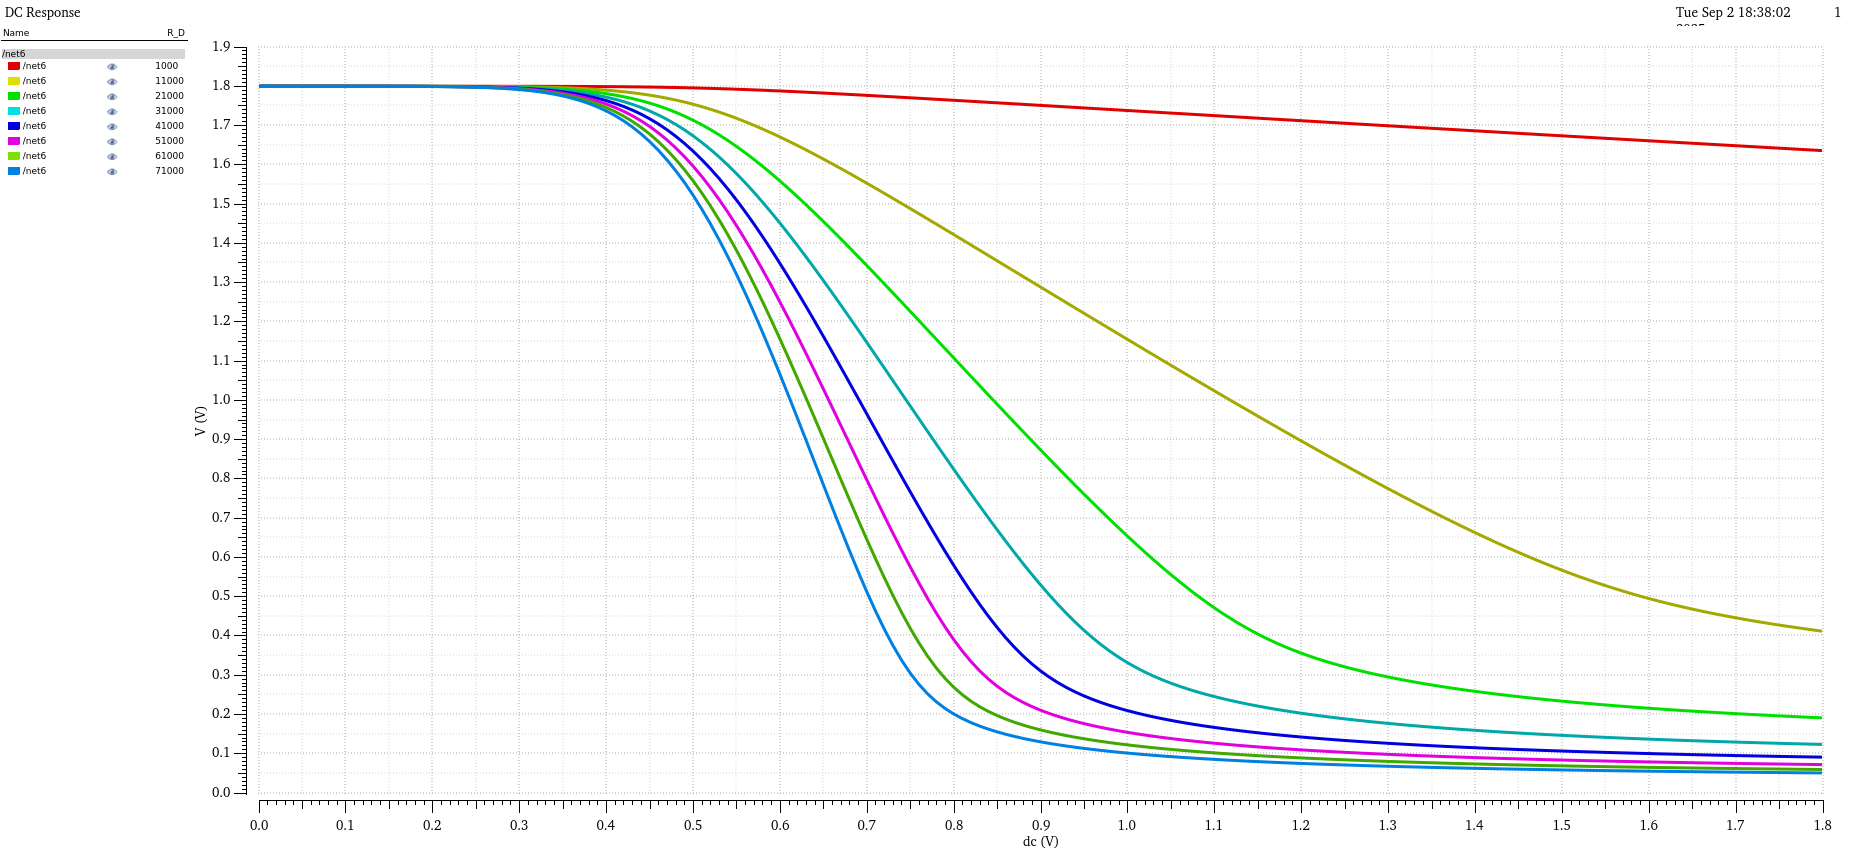
\includegraphics[width=\textwidth]{images/parameter-graph.png}
	\caption{Parametric VTC Curves}
	\label{fig:parametric_vtc}
\end{figure}

From Figure \ref{fig:parametric_vtc}, it can be seen that as the resistance increases, the VTC curve shifts to the left, and the bends where $V_{IH}$ and $V_{IL}$ are located also shift to the left. The noise margins also subseqnetly were lowered as the resistance increased. This is because as the resistance increases, the current through the NMOS decreases. 
This shift in the current causes the noise margins to change, and the overall noise margins change. 

Further analysis on this phenomenon regarding the effect of width and length on the noise margins can be done in future experiments.
\end{document}

